\chapter{Análise e Levantamento de Requisitos}
\label{chap:Analise-e-levantamento-de-requisitos}

\section{Análise de Produtos Semelhantes}
\label{sec:analise-de-produtos-semelhantes}

Um dos jogos que possui objetivos semelhantes ao do Caapora RPG e que coincidiu com a motivação do desenvolvimento é o jogo \textit{Pora: Free Cockatoos}

A\textit{Indonesian Society for Animal Welfare} (traduzido do inglês livre Sociedade Indonésio para o Bem Estar dos Animais)junto com outros desenvolvedores
criaram um aplicativo para conscientizar e educar em massa. “Muitas pessoas agora usam smartphones desde muito jovens”, diz Kinanti Kusumawardani, diretor executivo da \textit{Indonesian Society for Animal Welfare}. “Jogos para celular são um meio para chamar a atenção de maneira lúdica, uma vez que as pessoas parecem estar menos interessadas em ouvir palestras sobre o assunto”.

Para o desenvolvimento do jogo foi realizada uma competição em que os desenvolvedores deveriam criar um jogo que estimulasse a preservação da vida selvagem.

O Jogo \textit{Pora: Free Cockatoos} tem como personagem principal um peixe chamado Pora que possui um canhão onde ele lança torpedos aos caçadores que aprisionam as cacatuas.
Os vilões prendem as aves dentro de garrafas plasticas, uma pratica maldosa que realmente acontece.

“Os jogos podem fazer com que usuários se sintam envolvidos por uma causa sem que pareça algo muito sério”, afirmou Andi Surja Boediman, um parceiro da empresa que trabalha com os desenvolvedores. “É eficaz para promover a conscientização”. 

\begin{figure}[h!]
		\centering
		\Caption{\label{fig:exemplo-6} Jogo Pora: Free Cockatoos desenvolvido para conscientização dos mal tratos as aves da Indonésia}	
		\UECEfig{}{
			\fbox{
\includegraphics[width=9cm]{figuras/pora}}
		}{
			\Fonte{ANDA - Agencia de Noticias de Direitos Animais, 2015}
		}	
	\end{figure}
\pagebreak
\section{Requisitos do Sistema}
\label{sec:requisito-do-sistema}

\subsection {Requisitos Funcionais}

Foram definidos os seguintes requisitos funcionais, conforme exibido na Tabela 2:
\begin{table}[h!]	
	\centering
	\Caption{\label{tab:requiitos-funcionais}Requisitos Funcionais}	
	\IBGEtab{}{
		\begin{tabular}{cp{13cm}}
			\toprule
			Requisto & Função \\
			\midrule \midrule
			RF1 & O jogo deve ter um menu inicial contendo as seguintes opções: Iniciar Jogo e Opções. \\
			RF2 & Ao iniciar o jogo, o jogo deve apresentar um resumo sobre o cenário ao qual o jogador estará durante o jogo.\\
			RF3 & O jogo deve ter a opção de Pular o resumo do inicio do jogo.\\
			RF4 & A movimentação do personagem será controlada através do \textit{touchscreen} com controle direcional.\\
			R05 & Usuário terá a capacidade pegar o balde aguá quando tocado na tela do botão...\\
			RF6 & Usuário terá a capacidade jogar água no fogo apertando na tela o botão...\\
			RF7 & O jogo apresentará uma barra de vida do personagem Caapora que no qual ira diminuir toda vez que ele for 'queimado' \\
			RF8 & O balde devera ter uma barra de informação que mostrara o tanto de aguá que já foi enchido\\
			RF9 & Caso o usuário consiga apagar todo o fogo no tempo determinado, sera mostrada uma tela dizendo que o jogador conseguiu \\
			RF10 & Caso o usuário não consiga apagar todo o fogo em tempo determinado, sera mostrada uma tela dizendo que o jogador falhou\\
			
			\bottomrule
		\end{tabular}
	}{
	\Fonte{Elaborado pelo autor}
}
\end{table}

\subsection{Requisitos Não Funcionais}
Foram definidos os seguintes requisitos não funcionais, conforme exibido na Tabela 3:

\begin{table}[h!]	
	\centering
	\Caption{\label{tab:requisitos-nao-funcionais}Requisitos Não Funcionais}	
	\IBGEtab{}{
		\begin{tabular}{cp{13cm}}
			\toprule
			Requisito & Função \\
			\midrule \midrule
			RNF1 & O aplicativo deve funcionar na versão 3.0 do Android ou superior.\\
			RFN2 & O carregamento do jogo deve durar no máximo 10 segundos. \\
			RFN3 & A tela do dispositivo móvel deve ser \textit{touchscreen} e com tamanho minimo de XXX por XXXX\\
			
						\bottomrule
		\end{tabular}
	}{
	\Fonte{Elaborado pelo autor}
}
\end{table}

\section{Modelagem do Sistema}
\label{sec:modelagem-do-sistema}

A figura 19 apresenta o caso de uso do jogo, apresentando as ações que o jogador pode executar na aplicação.

\begin{figure}[h!]
		\centering
		\Caption{\label{fig:exemplo-} Caso de uso, ações do jogador}	
		\UECEfig{}{
			\fbox{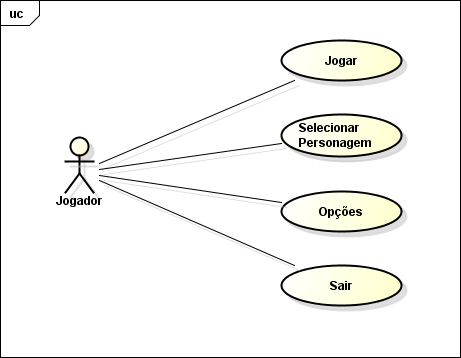
\includegraphics[width=13cm]{figuras/casodeuso}}
		}{
			\Fonte{Elaborado pelo autor}
		}	
	\end{figure}
\pagebreak


\begin{table}	
\centering
\Caption{\label{tab:caso-de-uso-jogar}Documentação do caso de uso Jogador}
\begin{tabular}{ | m{5cm} | m{8cm}| } 
\hline
\textbf {Nome do Caso de uso} & Jogar \\ 

\textbf {Ator Principal} & Jogador \\ 
\textbf {Resumo} & Esse caso de uso descreve as etapas percorridas por um jogador após ele selecionar a opção jogar \\
\textbf {Pré - condições} & Não se aplica\\
\hline
\textbf {Ações do Ator} & \textbf {Ações do Sistema}\\
\hline
1- O jogador seleciona a opção "Jogar" no menu principal. & 2 - Sistema exibe uma tela contendo uma mensagem informativa sobre o jogo.\\
3 - Jogador seleciona a opção "Pular" após ler as mensagens. & 4 - Sistema carrega o cenário do jogo.\\
\hline
\end{tabular}
\Fonte{Elaborado pelo autor}
\end{table}

\begin{table}	
\centering
\Caption{\label{tab:caso-selecionar-personagem}Documentação do caso de uso Selecionar Personagem}
\begin{tabular}{ | m{5cm} | m{8cm}| } 
\hline
\textbf {Nome do Caso de uso} & Selecionar Personagem \\ 

\textbf {Ator Principal} & Jogador \\ 
\textbf {Resumo} & Esse caso de uso descreve as etapas percorridas por um jogador durante a seleção de personagem \\
\textbf {Pré - condições} & Não se aplica\\
\hline
\textbf {Ações do Ator} & \textbf {Ações do Sistema}\\
\hline
1- O jogador seleciona a opção "Selecionar Personagem" na interface & 2 - Sistema exibe uma tela contendo personagens\\
3 - Jogador seleciona a personagem desejado & 4 - Sistema retorna para o menu principal.\\
\hline
\end{tabular}
\Fonte{Elaborado pelo autor}
\end{table}

\begin{table}	
\centering
\Caption{\label{tab:caso-de-uso-opcoes}Documentação do caso de uso Opções}
\begin{tabular}{ | m{5cm} | m{8cm}| } 
\hline
\textbf {Nome do Caso de uso} & Opções \\ 
\textbf {Ator Principal} & Jogador. \\ 
\textbf {Resumo} & Esse caso de uso descreve as etapas percorridas por um jogador após ele selecionar "Opções".\\
\textbf {Pré - condições} & Não se aplica.\\
\hline
\textbf {Ações do Ator} & \textbf {Ações do Sistema}\\
\hline
1- O jogador seleciona a opção "Opções" na interface & 2 - Sistema exibe uma tela contendo informações sobre áudio e vídeo.\\
3 - Jogador altera as configurações e salva & 4 - Sistema atualiza o jogo.\\
\hline
\end{tabular}
\Fonte{Elaborado pelo autor}
\end{table}

\begin{table}	
\centering
\Caption{\label{tab:caso-de-uso-sair}Documentação do caso de uso Sair}
\begin{tabular}{ | m{5cm} | m{8cm}| } 
\hline
\textbf {Nome do Caso de uso} & sair \\ 
\textbf {Ator Principal} & Jogador. \\ 
\textbf {Resumo} & Esse caso de uso descreve as etapas percorridas por um jogador após ele selecionar "Sair".\\
\textbf {Pré - condições} & Não se aplica.\\
\hline
\textbf {Ações do Ator} & \textbf {Ações do Sistema}\\
\hline
1- O jogador seleciona a opção "Sair" na interface & 2 - Sistema fecha o jogo..\\

\hline
\end{tabular}
\Fonte{Elaborado pelo autor}
\end{table}



\cite{Huetal2000} \lipsum[2] 

O autor \cite{lamport1986latex} e \cite{Maia2011} \lipsum[2] 







